\section{Atividade 1}
\subsection{Descrição do Modelo}
O sistema modelado é um oscilador massa-mola-amortecedor, onde a massa está sujeita à força restauradora de uma mola e ao amortecimento proporcional à velocidade. A equação diferencial que descreve o movimento do sistema é dada por:
\[
    m \ddot{x} + C \dot{x} + Kx = 0
\]
onde \( x \) representa o deslocamento da massa \( m \) da sua posição de equilíbrio, \( \dot{x} \) é a velocidade, \( \ddot{x} \) é a aceleração, \( C \) é o coeficiente de amortecimento, e \( K \) é a constante da mola. A força de entrada é considerada nula, indicando que não há forças externas atuando sobre o sistema após o instante inicial.

\subsection{Parâmetros do Sistema}
Os parâmetros utilizados no modelo do sistema são especificados como segue:
\begin{itemize}
    \item Massa (\( m \)): 10 kg
    \item Coeficiente de amortecimento (\( C \)): 7 Ns/m
    \item Constante da mola (\( K \)): 5 N/m
\end{itemize}

\subsection{Condições Iniciais para a Simulação}
As condições iniciais para a simulação são detalhadas na tabela a seguir, baseadas nos parâmetros especificados acima:
\begin{center}
    \begin{tabular}{|c|c|c|}
        \hline
        \textbf{Caso} & \textbf{Velocidade Inicial \( V_0 \)} & \textbf{Posição Inicial \( X_0 \)} \\
        \hline
        1             & \( 5 \, \text{m/s} \)                 & \( 0 \, \text{m} \)                \\
        2             & \( 0 \, \text{m/s} \)                 & \( 2.5 \, \text{m} \)              \\
        3             & \( 3.33 \, \text{m/s} \)              & \( 2 \, \text{m} \)                \\
        \hline
    \end{tabular}
\end{center}

Esta tabela reflete os valores numéricos para cada caso, facilitando a compreensão e a aplicação direta dos parâmetros na simulação.

\subsection{Código Scilab para simular a resposta do sistema massa-mola-amortecedor}
Código Scilab utilizado para as análises que serão feitas subsequentes
\begin{lstlisting}[language=Scilab, caption=Código Scilab para simular a resposta do sistema massa-mola-amortecedor]
    // Definicao das principais variaveis do sistema fisico
    m = 10;  // massa
    c = 7;   // coeficiente de amortecimento
    k = 5;   // constante da mola

    // Funcao que define o sistema de equacoes diferenciais (EDO) para o modelo massa-mola-amortecedor
    function dxdt = sistema(t, x)
    // x(1) representa o deslocamento, x(2) representa a velocidade
    // Esta funcao retorna a derivada da velocidade e do deslocamento, respectivamente
    dxdt = [x(2); -c/m * x(2) - k/m * x(1)];
    endfunction

    // Configuracao do intervalo de tempo para a simulacao
    t0 = 0; // Tempo inicial (s)
    tf = 20; // Tempo final (s)
    t = linspace(t0, tf, 1000); // Cria um vetor de tempo linearmente espacado para a simulacao

    // Definicao das condicoes iniciais para cada caso de simulacao
    condicoes_iniciais = [
    0, m/2;   // Caso 1: posicao inicial (m) e velocidade inicial (m/s)
    m/4, 0;   // Caso 2: posicao inicial (m) e velocidade inicial (m/s)
    m/5, m/3; // Caso 3: posicao inicial (m) e velocidade inicial (m/s)
    ];

    // Cores designadas para cada caso de simulacao para facilitar a visualizacao
    cores = ['#007bff', '#dc3545', '#8B4513']; // Azul, vermelho, marrom

    // Loop para executar e plotar cada caso de simulacao separadamente
    for i = 1:3
        x0 = condicoes_iniciais(i, :)'; // Transpoe as condicoes iniciais para a formatacao correta
        sol = ode(x0, t0, t, sistema); // Resolve a EDO usando o metodo de ODE

        scf(i); // Cria uma nova figura para cada iteracao
        plot(t, sol(1, :),  'color', cores(i),  'LineWidth', 2); // Plot do deslocamento x(t)
        xlabel('Tempo (s)'); // Etiqueta do eixo X
        ylabel('Deslocamento x(t)'); // Etiqueta do eixo Y
        title(['Resposta do Sistema para o Caso ', string(i)]); // Titulo do grafico
        legend('x(t)', "location", "best"); // Legenda
        xgrid(); // Ativa a grade no grafico
    end

    // Preparacao do grafico combinado
    scf(); // Cria uma nova figura
    clf(); // Limpa a figura atual
    xlabel('Tempo (s)');
    ylabel('Deslocamento x(t)');
    title('Resposta do Sistema para Todos os Casos');
    xgrid(); // Ativando a grade

    // Execucao da simulacao para cada caso e plotagem no mesmo grafico
    for i = 1:3
    x0 = condicoes_iniciais(i, :)'; // Condicoes iniciais para o caso i (transposto para coluna)
    sol = ode(x0, t0, t, sistema); // Resolvendo a equacao diferencial

    // Plotando os resultados com cores definidas
    plot(t, sol(1, :), 'color', cores(i), 'LineWidth', 2);
    end

    // Criar a legenda detalhando cada caso
    legend(['Caso 1: x0 = 0, v0 = m/2', 'Caso 2: x0 = m/4, v0 = 0', 'Caso 3: x0 = m/5, v0 = m/3'], "location", "best");
\end{lstlisting}

\subsection{Análise dos Resultados}
Cada um dos casos de simulação foi configurado com condições iniciais distintas para explorar como o sistema responde a diferentes estados iniciais de deslocamento e velocidade.

\subsubsection{Caso 1: Velocidade Inicial Elevada}
\begin{figure}[H]
    \centering
    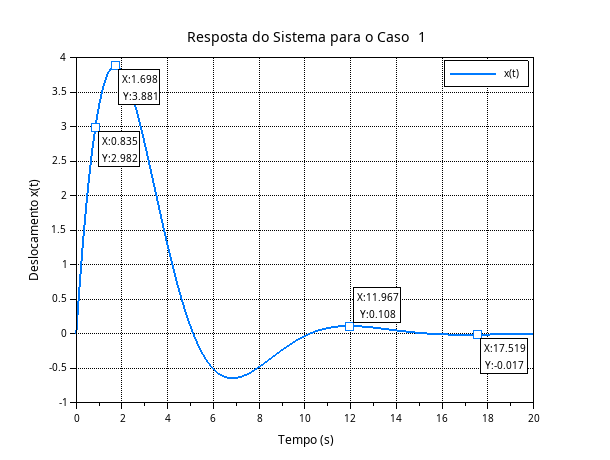
\includegraphics[width=0.6\textwidth]{atividades/1-atividade/assets/caso1.png}
    \caption{Resposta do sistema para o Caso 1}
\end{figure}
No Caso 1, o sistema é inicialmente impulsionado com uma alta velocidade (\(5 \, \text{m/s}\)), partindo do repouso (\(X_0 = 0\)). Esta condição inicial provoca uma resposta dinâmica vigorosa, onde a massa oscila com uma amplitude inicialmente elevada. O primeiro pico ocorre aproximadamente aos \(1.698 \, s\), alcançando uma altura de \(3.881 \, m\). Este pico representa a conversão máxima da energia cinética inicial em energia potencial. A subsequente queda rápida na amplitude das oscilações, como observado nos pontos seguintes, ilustra o efeito do amortecimento significativo (\(C = 7 \, \text{Ns/m}\)). Este amortecimento não só rapidamente reduz a amplitude das oscilações, mas também garante que o sistema estabilize rapidamente, evitando oscilações prolongadas e retornando ao equilíbrio em aproximadamente \(17.519 \, s\), como indicado pelo deslocamento quase nulo (\(-0.017 \, m\)).

\subsubsection{Caso 2: Deslocamento Inicial Sem Velocidade}
\begin{figure}[H]
    \centering
    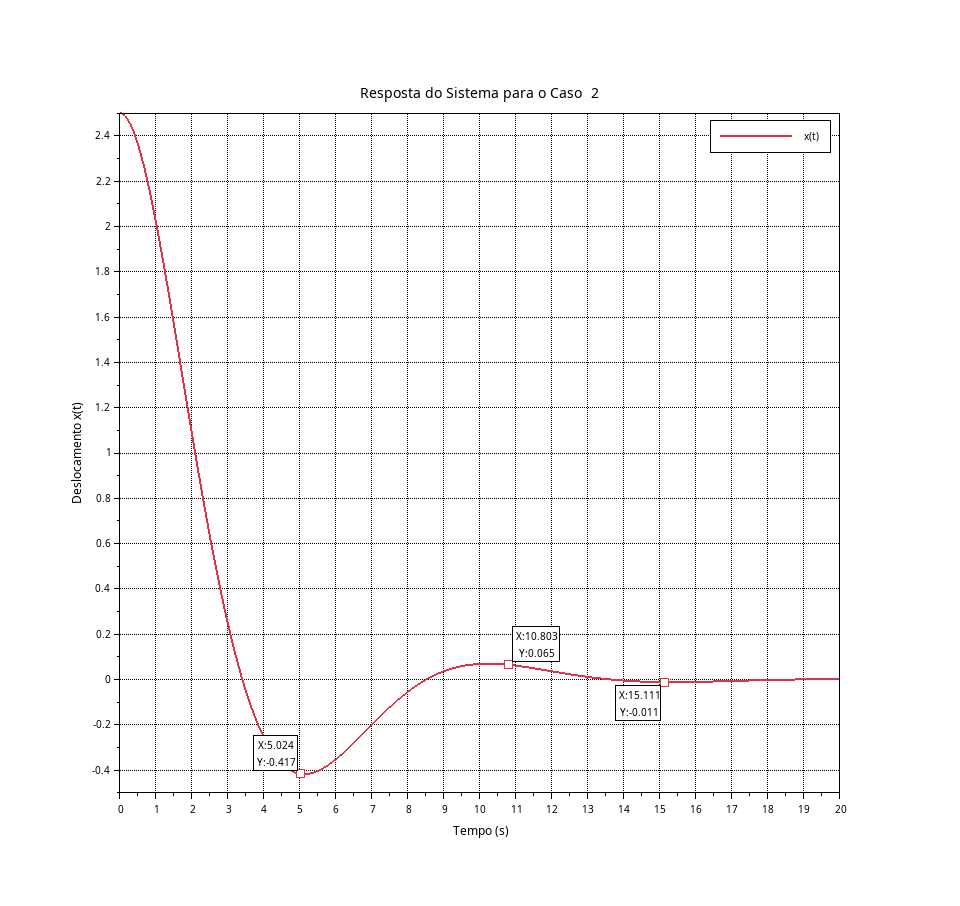
\includegraphics[width=0.6\textwidth]{atividades/1-atividade/assets/caso2.png}
    \caption{Resposta do sistema para o Caso 2}
\end{figure}
O Caso 2 é caracterizado por um deslocamento inicial de \(2.5 \, \text{m}\) sem impulso inicial de velocidade (\(V_0 = 0\)). A resposta do sistema é a de um oscilador subamortecido. Iniciando de um ponto de deslocamento máximo, o sistema mostra uma rápida resposta inicial seguida de oscilações que decaem progressivamente em amplitude. O primeiro pico de deslocamento negativo ocorre aproximadamente aos \(5.057 \, s\), com um deslocamento de \(-0.417 \, m\). Esta condição inicial destaca como a energia potencial armazenada na mola é inicialmente convertida em energia cinética, que é gradualmente dissipada pelo amortecedor. As oscilações subsequentes mostram uma diminuição gradativa na amplitude, com o sistema aproximando-se do equilíbrio em torno de \(15.026 \, s\), ilustrando uma transferência de energia mais prolongada e uma estabilização gradual em comparação ao Caso 1.

\subsubsection{Caso 3: Velocidade e Deslocamento Iniciais}
\begin{figure}[H]
    \centering
    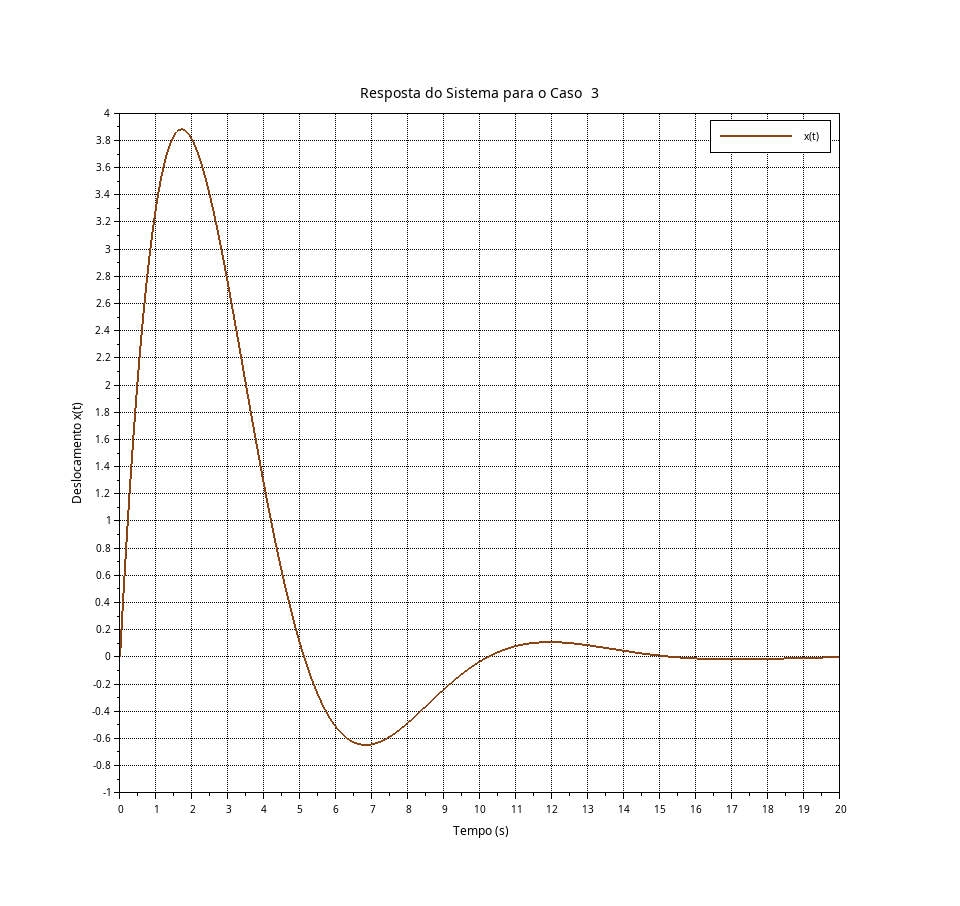
\includegraphics[width=0.6\textwidth]{atividades/1-atividade/assets/caso3.png}
    \caption{Resposta do sistema para o Caso 3}
\end{figure}
No Caso 3, o sistema inicia com condições iniciais moderadas tanto de velocidade (\(3.33 \, \text{m/s}\)) quanto de deslocamento (\(2 \, \text{m}\)). Esta configuração produz uma resposta dinâmica complexa, onde a interação entre energia cinética e potencial é claramente visível. O primeiro pico de amplitude ocorre em \(t \approx 1.241 \, s\) com um deslocamento de \(3.873 \, m\), ilustrando a conversão da energia cinética inicial em potencial. Posteriormente, as oscilações decrescem rapidamente em amplitude devido ao amortecimento significativo, estabilizando-se próximo de zero em \(t \approx 16.645 \, s\). As oscilações são mais persistentes e menos intensas do que nos outros casos, refletindo um equilíbrio dinâmico entre as energias cinética e potencial ao longo da simulação.

\subsubsection{Comparação Unificada dos Casos}
\begin{figure}[H]
    \centering
    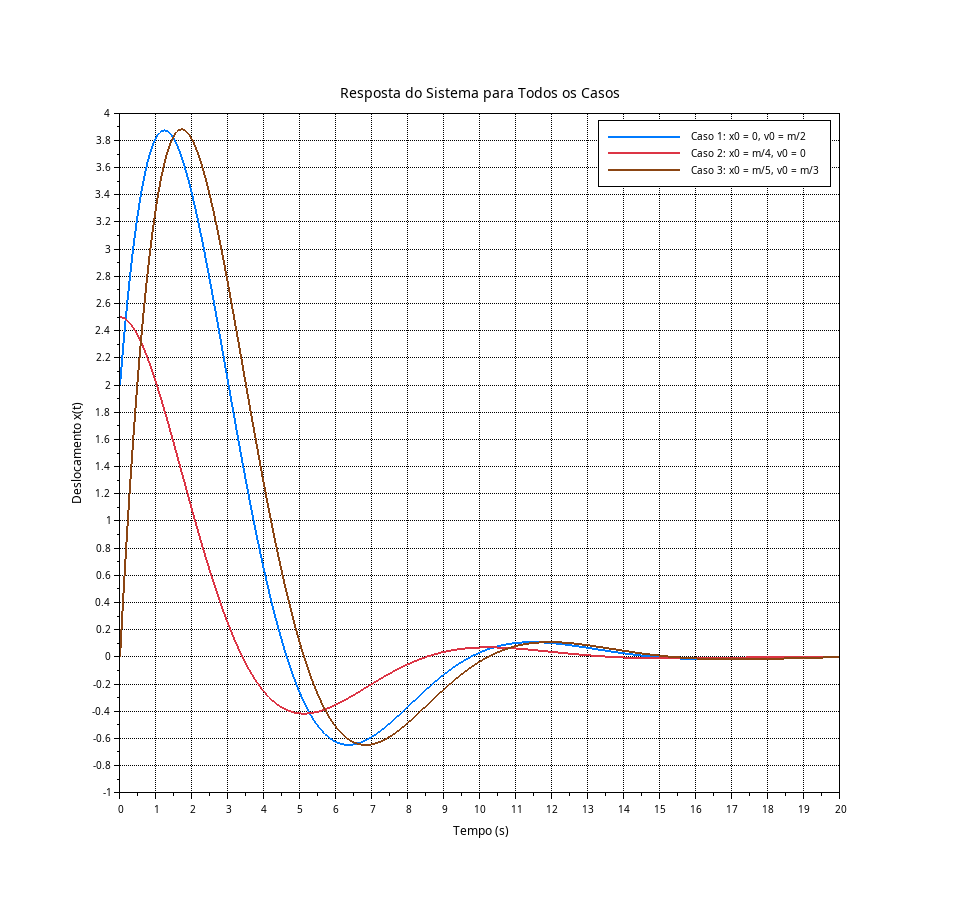
\includegraphics[width=0.6\textwidth]{atividades/1-atividade/assets/caso-all-in-one.png}
    \caption{Resposta unificada do sistema para os Casos 1, 2 e 3}
\end{figure}
A análise unificada dos três casos demonstra de forma clara as diferenças significativas nas respostas do sistema decorrentes de diversas condições iniciais. A seguir, discutiremos detalhadamente cada resposta e suas implicações para a compreensão do comportamento dinâmico do sistema:

\begin{itemize}
    \item \textbf{Caso 1 (Azul Escuro)}: Iniciado com uma alta velocidade inicial (\(5 \, \text{m/s}\)) e sem deslocamento inicial, este caso exibe a maior amplitude de oscilação observada, com um pico inicial em \(t \approx 1.256 \, s\) e \(x \approx 3.873 \, m\). A energia cinética inicial é rapidamente convertida em energia potencial pela mola, resultando em oscilações de grande amplitude que são rapidamente amortecidas, aproximando-se de um estado de equilíbrio em \(t \approx 17.389 \, s\). Este caso ilustra o efeito de um forte amortecimento, onde a energia é dissipada rapidamente, levando a um retorno rápido à posição de equilíbrio sem oscilações residuais prolongadas.

    \item \textbf{Caso 2 (Vermelho)}: Com um deslocamento inicial (\(2.5 \, \text{m}\)) e sem velocidade inicial, o sistema mostra uma resposta clássica de um oscilador subamortecido. A energia potencial armazenada na mola é convertida gradualmente em energia cinética, com a energia sendo dissipada ao longo do tempo pelo amortecedor. As oscilações decaem suavemente, com a primeira oscilação significativa cruzando o zero em \(t \approx 7.006 \, s\) e um deslocamento de \(-0.587 \, m\), refletindo uma conversão mais lenta de energia que é típica em aplicações onde é necessário manter uma certa quantidade de movimento ou onde oscilações graduais são preferíveis.

    \item \textbf{Caso 3 (Marrom)}: Este caso combina condições iniciais moderadas de velocidade (\(3.33 \, \text{m/s}\)) e deslocamento (\(2 \, \text{m}\)), resultando numa resposta dinâmica mais complexa que engloba características dos dois primeiros casos. A amplitude inicial é significativa, com um pico inicial em \(t \approx 1.241 \, s\) e \(x \approx 3.873 \, m\). As oscilações são mais controladas e decaem de maneira gradual, aproximando-se de um estado estável em \(t \approx 16.645 \, s\). Este caso destaca a importância do equilíbrio entre rigidez da mola e amortecimento no projeto de sistemas mecânicos, onde é necessário um compromisso entre estabilidade rápida e manutenção de energia dinâmica.
\end{itemize}

Esta comparação detalhada destaca a influência das condições iniciais na resposta do sistema e também o papel crítico do amortecimento e da rigidez da mola na determinação da natureza da resposta dinâmica. A análise fornece insights valiosos para o design e a otimização de sistemas mecânicos em engenharia, sublinhando a necessidade de uma seleção cuidadosa de parâmetros de acordo com os requisitos específicos de cada aplicação.

\subsection{Comentários Gerais e Conclusão}
Os gráficos e análises ilustram claramente como as condições iniciais impactam a resposta dinâmica do sistema massa-mola-amortecedor. A energia inicial, seja como deslocamento ou velocidade, define a resposta imediata do sistema, mostrando a complexidade do comportamento de sistemas dinâmicos lineares. Observamos que o amortecimento é essencial para reduzir as oscilações e trazer o sistema de volta ao repouso de maneira eficiente, sublinhando sua importância no design de componentes mecânicos.

A adequação do coeficiente de amortecimento e da rigidez da mola é crucial para otimizar sistemas para suas funções específicas, como a absorção de choques em suspensões de veículos ou a precisão em instrumentos de medição. Além disso, a análise das condições iniciais é vital no planejamento e teste de sistemas mecânicos, onde engenheiros e designers devem antecipar cenários variados de operação.

Este estudo destaca a necessidade de um entendimento profundo das dinâmicas de sistemas para inovação em engenharia, proporcionando uma base sólida para a compreensão dos princípios de mecânica e dinâmica que são fundamentais no design de sistemas controlados e mecanismos em geral.
